\chapter{Conceptual Design}
\label{sec:design}
%
\todo{Describe Chapter}


% ===========================================
% ===========================================
\section{Cluster Architecture}

\begin{figure}[h]%
\centering
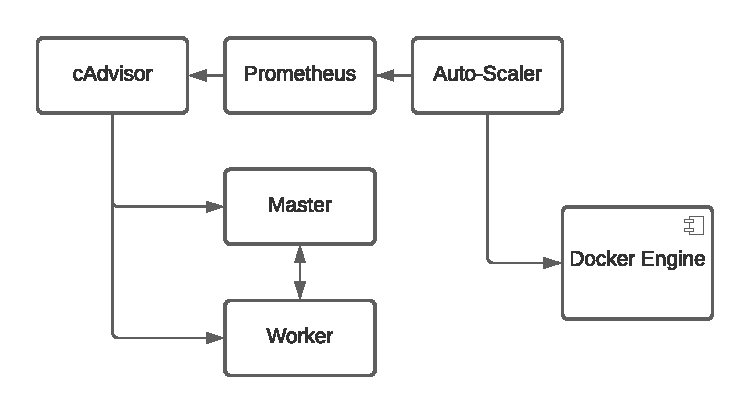
\includegraphics[scale=0.8]{images/04_conceptual_design/cluster_architecture/overall_architecture}%
\caption{Scaling process UML activity model - Source: Authors own model.}%
\label{fig:ca-overall_architecture}%
\end{figure}

% Cluster consists of
The cluster conists of multiple components runnin in a own docker container. Prometheus, cAdvisor, Spark Master, Spark Worker, Auto-Scaler.
% Communication between components
cAdvisor collects metrics from all available docker container running in the same network. Prometheus scrapes metrics from cAdvisor and stores them as time-series-data in its ts-db. The Auto-Scaler read metric from Prometheus via its REST API. If a scaling action is necessary the auto-scaler scales the number of worker.
% 


% ===========================================
% ===========================================
\section{DevOps Process}


% ===========================================
% ===========================================
\section{Autonomic Manager}
% Short description of old section
As described in section ABC, the Autonomic Manager follows the MAPE Architecture. The Autonim manager implements a Loops which is responsible for collecting and analyzing the metrics.


\subsection{Workflow}
% Process figure
\begin{figure}[h]%
\centering
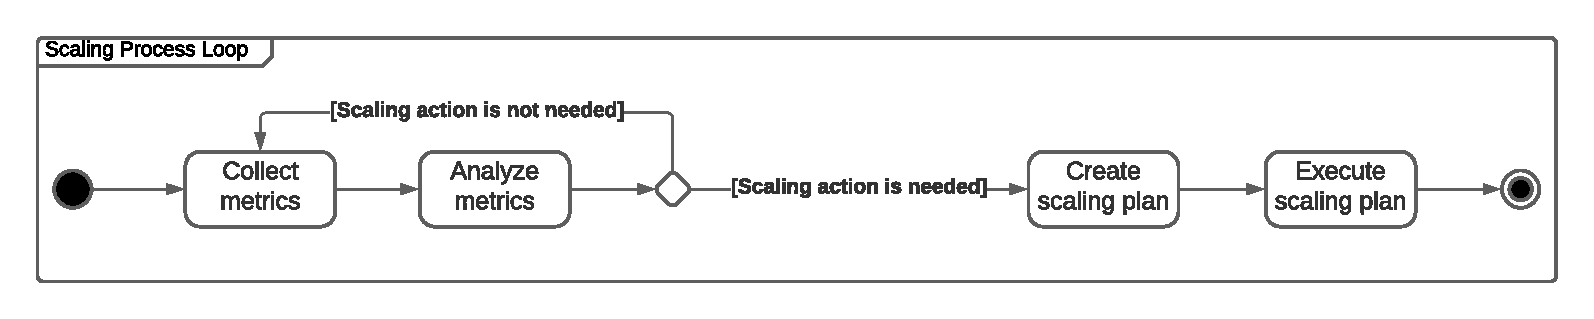
\includegraphics[scale=0.6]{images/04_conceptual_design/01_scaling_process_model}%
\caption{Scaling process UML activity model - Source: Authors own model.}%
\label{fig:am-workflow-process_model}%
\end{figure}

% Whats is the workflow/meaning

% How is the workflow structured
As illustrated in \Fig{fig:am-workflow-process_model} the workflow consists of four different steps:

\begin{enumerate}
\item Collect metrics
\item Analyze metrics
\item Create scaling plan
\item Scale environment
\end{enumerate}

In the first step, all metrics (described in \SubSec{subsec:design-metrics}) are collected using cAdvisor and will be stored in Prometheus. The autonomic manager (described in \Sec{sec:design-manager}) gathers all metrics from Prometheus REST API and analyzes the data to discover if scaling actions are necessary. According to the data, the manager creates a plan to estimate how many nodes needed to be added or removed. In the last step, the scaling plan will be executed by the manager.

% Wie werden Metriken gesammelt
% Wie werden Metriken analysiert
% Wei wird der Manager benachrichtigt
% Wie wird skaliert
% Die Loop implementiert die loop von autonomous computing MAPE


\subsection{Design}

% Component design
\begin{figure}[h]%
\centering
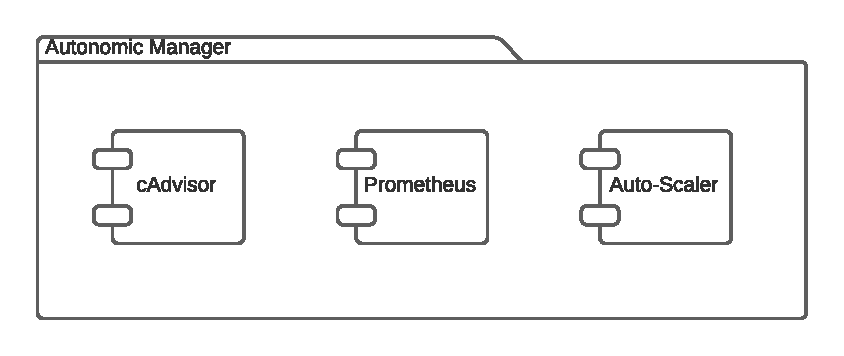
\includegraphics[scale=0.6]{images/04_conceptual_design/autonomic_manager/design}%
\caption{Scaling process UML activity model - Source: Authors own model.}%
\label{fig:am-design-component}%
\end{figure}

The autonomic manager will be compose by several components to build a manager. To collect the metrics, cAdvisor will be used (see Section A), for storing the metrics Prometheus will be used (see Section B) and for auto-scaling, a Auto-scaler will be developed.


\section{Auto-Scaler}
% What is the Auto-Scaler
The Auto-Scaler is a component of the the Autonomic Manager and is responsible for the Analyze, Plan and Execution phase.
% Complete autonomic manager
Together with cAdvisor and Prometheus, the Auto-Scaler builds a complete Autonomic Manager according to the architecture demonstrated in \SubSec{subsec:background-autonomic_computing-autonomic_manager}.
% controll loop
In addition, the Auto-Scaler implements the control-loop which is responsible to make adjustments in the environment.

% HIER NOCH BILD VON SCALER WIE MIT DER MAPE ARCH


\subsection{Configuration}
\label{subsec:design-auto_scaler-configuration}
The Auto-Scaler needs specific configuration properties to be able to collect the correct metrics from Prometheus and deploy new Apache Spark worker container in the environment. The following are properties that have to be defined to ensure that the Auto-Scaler is able to collect meaningful metrics and scale Apache Spark worker as expected.

\subsubsection{General properties}

\begin{itemize}
\item \textbf{Interval seconds:} The number of seconds when the loop has to repeat needs to be defined.
\end{itemize}

\subsubsection{Apache Spark worker properties}

\begin{itemize}
\item \textbf{Worker image:} To guarantee that each Spark worker is homogeneous, all worker container should be created with the same image.

\item \textbf{Worker network:} To establish communication between all Spark worker and the Spark master, all new Spark worker container should be in the same network.

\item \textbf{Worker thresholds:} The minimum and maximum number of concurrent Spark worker should be defined. To avoid the cold start effect, the minimum amount of worker should be 1. \todo{CHeck nochmal den Cold Start effekt}

\item \textbf{Apache Spark master URI:} To distribute the workload across all Spark Worker, all Spark Worker need to communicate with the Spark master.
\end{itemize}

\subsubsection{Prometheus properties}

\begin{itemize}
\item \textbf{Prometheus URL:} The Auto-Scaler will collect the configured metrics from Prometheus REST API.

\item \textbf{Prometheus query:} A PromQL query needs to be defined to collect specific metrics for CPU utilization calculation. 
\end{itemize}


\subsection{Analyze}
% Short intro to analyze phase
In order to determine if a scaling-action is necessary, the Auto-Scaler has to analyze the collected metrics. 
% Hier scaling heat algorithmus bla bla
The Auto-Scaler will use the Scaling Heat algorithm (described in Section BLA) to analyze metrics.

\subsection{Plan}
% Short intro
If a scaling-action is necessary, Spark worker container have to be created or removed from the environment. 
% MinMax CPU GPU utilization
The percentage of minimum and maximum CPU and GPU utilization across all Spark worker have to defined (described in \SubSec{subsec:design-auto_scaler-configuration}). These are the goals that the Auto-Scaler tries to achieve.
% MinMax Spark Worker
In addition, the minimum and maximum amount of concurrent Spark Worker have to be set (described in \SubSec{subsec:design-auto_scaler-configuration}) to guarantee that not too many or less Spark Worker are running at the same time HIER IST SEHR SCHWAMMIG; GUCK MAL IN DIE PAPER.
%
To achieve the defined goals of CPU and GPU utilization as well as ensure that the minimum and maximum number of concurrent Spark worker is observed, the Auto-Scaler will use the KHPA algorithm (described in Section BLA).


% ===========================================
% ===========================================
\section{Metrics}
% Welche metrics gibt es
% Welche metrics werden gesammelt (nur von den Worker)
% Wie werden die metrics berechnet

\subsection{CPU Utilization}
% Evtl ist hier der faösche platz -> Besser eine Metrics section wo erklärt wird, wie das berechnet werden soll.
\todo{Hier auf Tabelle verweisen (Anhang) Metriken die von Prometheus + cAdvisor bereitgestellt werden}

% How is the CPU Utilization being calculated
To adapt to business needs, the CPU percentage of each Spark Worker will be calculated. Prometheus provides several metrics to calculate the CPU percentage. The CPU percentage of all Worker can be calculated as follows:

% Ist nicht ganz korrekt, muss ja irgendwie noch durch die Anzahl an Worker geteilt werden
\begin{equation}
CPUUtilization = \sum ContainerCPUUserSecondsTotal \times 100 / NumberOfWorker
\label{eq:formel}
\end{equation}


\subsection{GPU Utilization}

